\chapter{The MakerFluidics Framework}
\label{chapter:mf}
\thispagestyle{myheadings}

% set this to the location of the figures for this chapter. it may
% also want to be ../Figures/2_Body/ or something. make sure that
% it has a trailing directory separator (i.e., '/')!
\graphicspath{{2_MakerFluidics/Figures/}}

\section{Introduction}
\label{sec:mfIntro}

MakerFluidics is a microfluidic fabrication and control framework that operates within a set of constraints guided by the ideals of automation and the modern ``maker movement''. This framework integrates into the larger microfluidic design flow shown in Figure \ref{fig:fullflow}, but it can also be employed on its own. MakerFluidics accepts physical and temporal valve control requirements and a microfluidic device design as inputs and provides the necessary control software, manufacturing files and assembly information required to build a self-contained microfluidic device and control infrastructure.

\section{Problem Statement}
\label{sec:mfPS}
A significant aim of the modern maker movement is to make technology and technological ``know-how'' accessible to the masses. One way to accomplish this goal is to devise solutions using resources that are flexible and ubiquitous \cite{schrock2014education}. A significant criticism often levied against the field of microfluidics is its high barrier to entry often as a result of the need for highly specialized fabrication and control equipment as well as expertise that is typically found only in labs dedicated to microfabrication \cite{whitesides2006}. This work seeks to create a design-to-device, automated microfluidic work-flow constrained by the ideals espoused in maker culture. 

\begin{figure}[h]
  \begin{minipage}[t]{0.99\linewidth}\centering
    \includegraphics[width=14cm]{fullflow.pdf}
    \medskip
  \end{minipage}\hfill
  \caption[Microfluidic specify--design--build workflow]{MakerFluidics is part of a larger microfluidic design flow that spans from biological specification to microfluidic fabrication and control}
    \label{fig:fullflow}
\end{figure}


\section{Contstraints}
\label{sec:mfConstraints}
An important goal of the maker movement is to increase technology's accessibility. This ideal is levied on MakerFluidics in the form of a series of constraints, the first of which is that all fabrication equipment must be sourced through ubiquitous consumer and retail product outlets such as Amazon.com in the Unites States, or Amazon.ca, .co.uk, .jp, etc. internationally, and each individual piece of equipment required for fabrication and control must cost less than \$100. A desktop computer numerical control (CNC) mill and 3D printer are excepted from this constraint on the basis that they are common maker-space tools with a wide variety of uses extending well beyond the field of microfluidics; the cost of the CNC mill (Othermill, Othermachine Co.) and 3D printer (Ultimaker 2, Ultimaker B.V.) used in our lab are each less than \$2,500. Additionally, all elements of the complete software tool chain must be free and/or open-source. 

To further facilitate microfluidic accessibility, all fabrication and control protocols must be accomplished without specialized infrastructure beyond a wall electrical outlet. This excludes fume hoods, clean room facilities, tank storage, vacuum lines and corona/plasma bonders. The process for designing, fabricating and controlling programmable (i.e., valved) microfluidics within the specified constraints is explored. Each stage of the process includes a comparison of current methods to methods developed or adopted by the MakerFluidics framework. 

\begin{table}[H]
% table caption is above the table
\caption[Infrastructure requirements for soft lithography versus MakerFluidics]{Necessary infrastructure to perform soft lithography versus that required for MakerFluidics.}
\label{tab:mfInf}       % Give a unique label
% For LaTeX tables use
\centering
\begin{tabular}{lcc}
\hline\noalign{\smallskip}
Infrastructure & MakerFluidics & Soft Lithography\\
\noalign{\smallskip}\hline\noalign{\smallskip}
Clean Room & Not Required & Required \\
Fume Hood & Not Required & Required \\
Vacuum Line & Not Required & Required \\
Tank Storage & Not Required & Required \\
Electrical Outlet & Required & Required \\
Equipment Overhead & ~\$4,000 & ~\$80,000 \\
\noalign{\smallskip}\hline
\end{tabular}
\end{table}


\section{Microfluidic Design}
\label{sec:mfDesign}

Three levels of software are required to design and fabricate a novel chip geometry using a CNC micromill: a computer aided design (CAD) tool is used to create a solid model of the device; computer aided manufacturing (CAM) software generates the commands (also called toolpaths) that are sent directly to the micromill; and control software manages the connection between a computer and the micromill and sends individual toolpaths to the micromill. 

Device designs were created using OpenSCAD \cite{wikiOpenScad}, a free and open source CAD tool that reads script files to generate solid models. The ability to describe a solid model using only text is an important distinction between OpenSCAD and typical 3D modeling software packages (ex., AutoCAD, SolidWorks, etc.), which often require geometries to be manually drawn. Text-based modeling allows for automatic generation of device designs using a CAD workflow, such as that shown in Figure \ref{fig:fullflow}. MakerFluidics leverages OpenSCAD by creating device primitives that are stored in custom libraries. As shown in Listing \ref{lst:XposerChip}, these primitives are parametric, allowing them to be ``called'' in a fashion similar to that of an object-based programming language. 

\begin{minipage}{0.95\linewidth}
\centering 
	\begin{lstlisting}[caption={This single line of OpenSCAD creates the 3D model shown in Figure \ref{fig:mfParams}(A). Once a primitive is defined in OpenSCAD, the parameters associated with each device geometry can be modified and the corresponding solid model will adjust to reflect the changes.},label={lst:XposerChip}, frame=single, language=scad]
  transposerNet(N=3, w_channel=1, r_valve=1, scale_x = 1);
\end{lstlisting}
\end{minipage}

Once a solid model is created using a CAD tool, the solid model must be imported by CAM software in order to generate the toolpaths that will be sent to the mill. MakerFluidics uses Autodesk Fusion 360 to create toolpaths for 3D models, such as mesh models (ex., an STL file). All three CNC mills tested in the lab (Othermill V2 by Othermachine Co.; Othermill Pro by Othermachine Co.; and Nomad 883 by Carbide 3D) have machine-specific control software with the capability to directly process 2D models, such as a vector-graphics file (ex., an SVG file). All of the CAM software listed above is free, but not necessarily open source. A standard operating procedure for interacting with Fusion 360 in order to generate toolpaths and operate the Othermill V2 or the Othermill Pro can be found in Appendix \ref{appendix}.


\begin{figure}[h]
  \begin{minipage}[t]{0.99\linewidth}\centering
    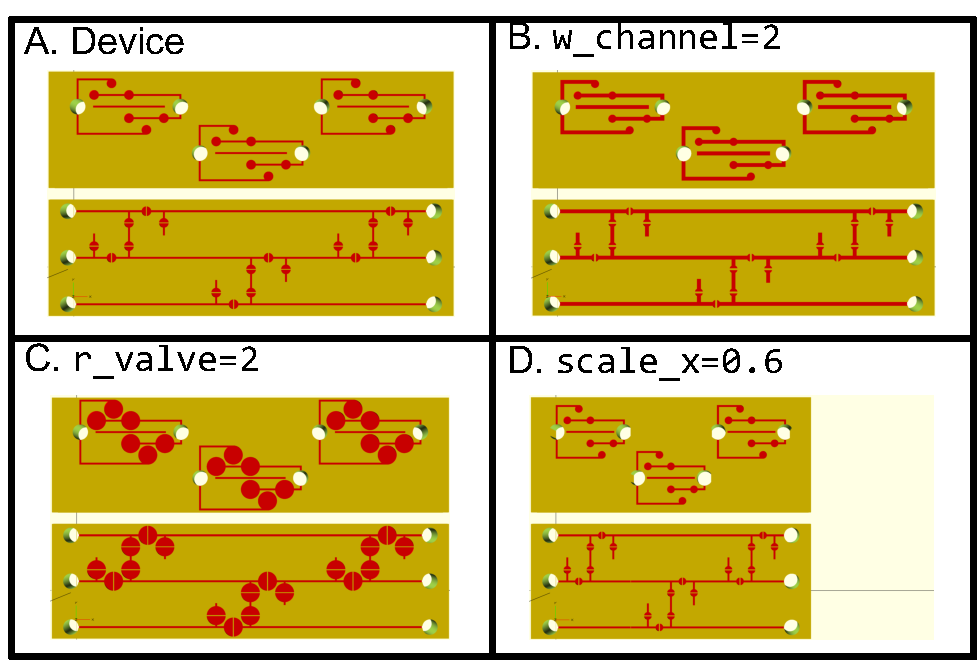
\includegraphics[width=14cm]{params.pdf}
    \medskip
  \end{minipage}\hfill
  \caption[Example device parameters]{Example parameters associated with a network of transposer primitives. The primitive and routing topology are presented in detail in Chapter \ref{chapter:xposer}. (A) shows the baseline device. (B) illustrates modifying the channel parameter to make the channels wider. (C) shows how the valve dimensions can be modified using a parameter associated with valve radius. (D) shows how the entire device can scale in the x-dimension using yet another parameter.}
    \label{fig:mfParams}
\end{figure}

\section{Microfluidic Fabrication}
\label{sec:mfFabrication}
The fabrication of a microfluidic device typically has two main steps: pattern geometries and seal layers \cite{mcdonald2002poly}.

\subsection{Pattern Geometries}
Channel and valve geometries are etched in thermoplastic polymers using a desktop CNC mill. This stands in sharp contrast from conventional methods of microfluidic fabrication, namely photolithography and wet etching, which require the use of clean room facilities and highly specialized equipment. The CNC approach is well-suited for integrating valving technologies such as monolithic membrane valves \cite{grover2003monolithic} (Figure \ref{fig:valves}) and centrifugal capillary valves \cite{madou1998labcd}. A significant trade-off for the relative ease of CNC milling thermoplastics using a desktop (i.e., not industrial-grade) CNC mill is that the maximum resolution is ~25$\mu$m with an exponential increase in reliability seen at feature sizes greater than 250$\mu$m \cite{guckenberger2015micromilling}, whereas microfluidic geometries using conventional methods such as photolithography can reliably achieve features smaller than 1$\mu$m \cite{mcdonald2002poly}.

\begin{figure}[h]
  \begin{minipage}[t]{0.99\linewidth}\centering
    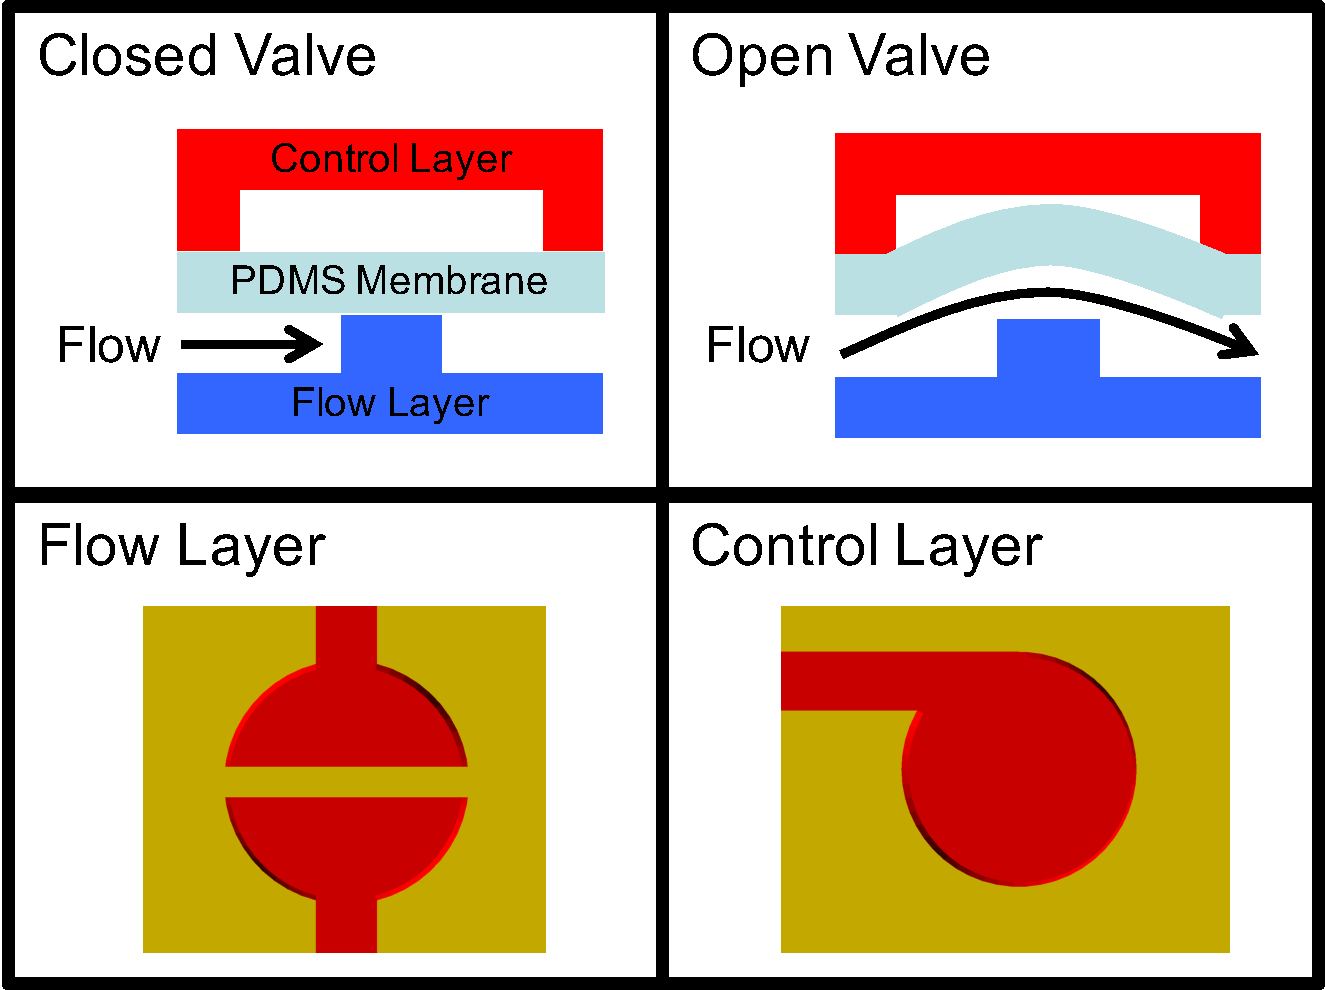
\includegraphics[width=14cm]{valves1.pdf}
    \medskip
  \end{minipage}\hfill
  \caption[Illustration of valving primitive]{Normally-closed monolithic membrane valves \cite{grover2003monolithic} are realized by introducing discontinuities in the flow layer (blue) and a corresponding pneumatic cavity in the control layer (red). These two layers are separated by a PDMS membrane. To open the valve a vacuum is introduced into the cavity in the control layer.}
    \label{fig:valves}
\end{figure}

\begin{table}[H]
% table caption is above the table
\caption[Dimensional constraints of soft lithography versus MakerFluidics]{Published dimensional constraints regarding devices fabricated using the MakerFluidics protocol versus that of soft lithography. Aspect Ratio is defined as feature height to feature width.}
\label{tab:mfDims}       % Give a unique label
% For LaTeX tables use
\centering
\begin{tabular}{p{2cm}ccp{4cm}}
\hline\noalign{\smallskip}
Dimension & MakerFluidics & Soft Lithography & Reference \\
\noalign{\smallskip}\hline\noalign{\smallskip}
\multirow{2}{*}{Aspect Ratio} & Tool Dependant & \multirow{2}{*}{1:20} & \cite{schaller1999microstructure}\\ 
& (often 3:1) & & \cite{qin2010soft}{\smallskip}\\
  \hline\noalign{\smallskip}
Minimum & Tool Dependant & \multirow{3}{*}{$<$1$\mu$m} & \cite{sweatt2008diamond}\\ 
Feature & (25$\mu$m Demonstrated) & & \cite{qin2010soft}\\
Size & (5$\mu$m Theoretical) & & {\smallskip}\\
  \hline\noalign{\smallskip}
  Minimum & \multirow {3}{*}{25$\mu$m} & \multirow{3}{*}{$<$1$\mu$m} & \cite{yen2016cost}\\ 
Feature & & & \cite{qin2010soft}\\
Spacing & & & {\smallskip}\\
  \hline\noalign{\smallskip}
  Bonding Capacity & \multirow{2}{*}{5 psi} & \multirow{2}{*}{50 psi} & \cite{mcdonald2002poly}{\smallskip}\\
  \hline\noalign{\smallskip}
\multirow{3}{*}{Materials} & Thermoplastics & PDMS & \cite{schaller1999microstructure}\\
& Soft Metals & Silicon & \cite{qin2010soft}\\
& Cured Thermosets & & \\
\noalign{\smallskip}\hline
\end{tabular}
\end{table}


\subsection{Seal Layers}
Once geometries are etched into the desired substrate, sealing these channels becomes the next challenge. Polydimethylsiloxane (PDMS) is a common material for fabricating microfluidics \cite{mcdonald2002poly} and is also commonly used to encapsulate solar panels and outdoor lighting. It is because of the latter property that PDMS (Sylgard 184, Dow Corning) is available through retail outlets, such as Amazon, and, thus, falls within the constraints for adoption by the MakerFluidics fabrication paradigm. PDMS can be sealed irreversibly through modifications to its surface chemistry via plasma or corona exposure or sealed reversibly simply using the material's inherent Van der Waals attraction to various materials including itself, glass and thermoplastics \cite{mcdonald2002poly}. Since irreversible sealing through surface treatments involves specialized machinery, MakerFluidics employs the latter method via Van der Waals force. The trade-off being that the reversible seal cannot withstand pressures greater than 5psi \cite{mcdonald2002poly}. The entire protocol is summarized in Figure \ref{fig:fabFlow}.


\begin{figure}[h]
  \begin{minipage}[t]{0.99\linewidth}\centering
    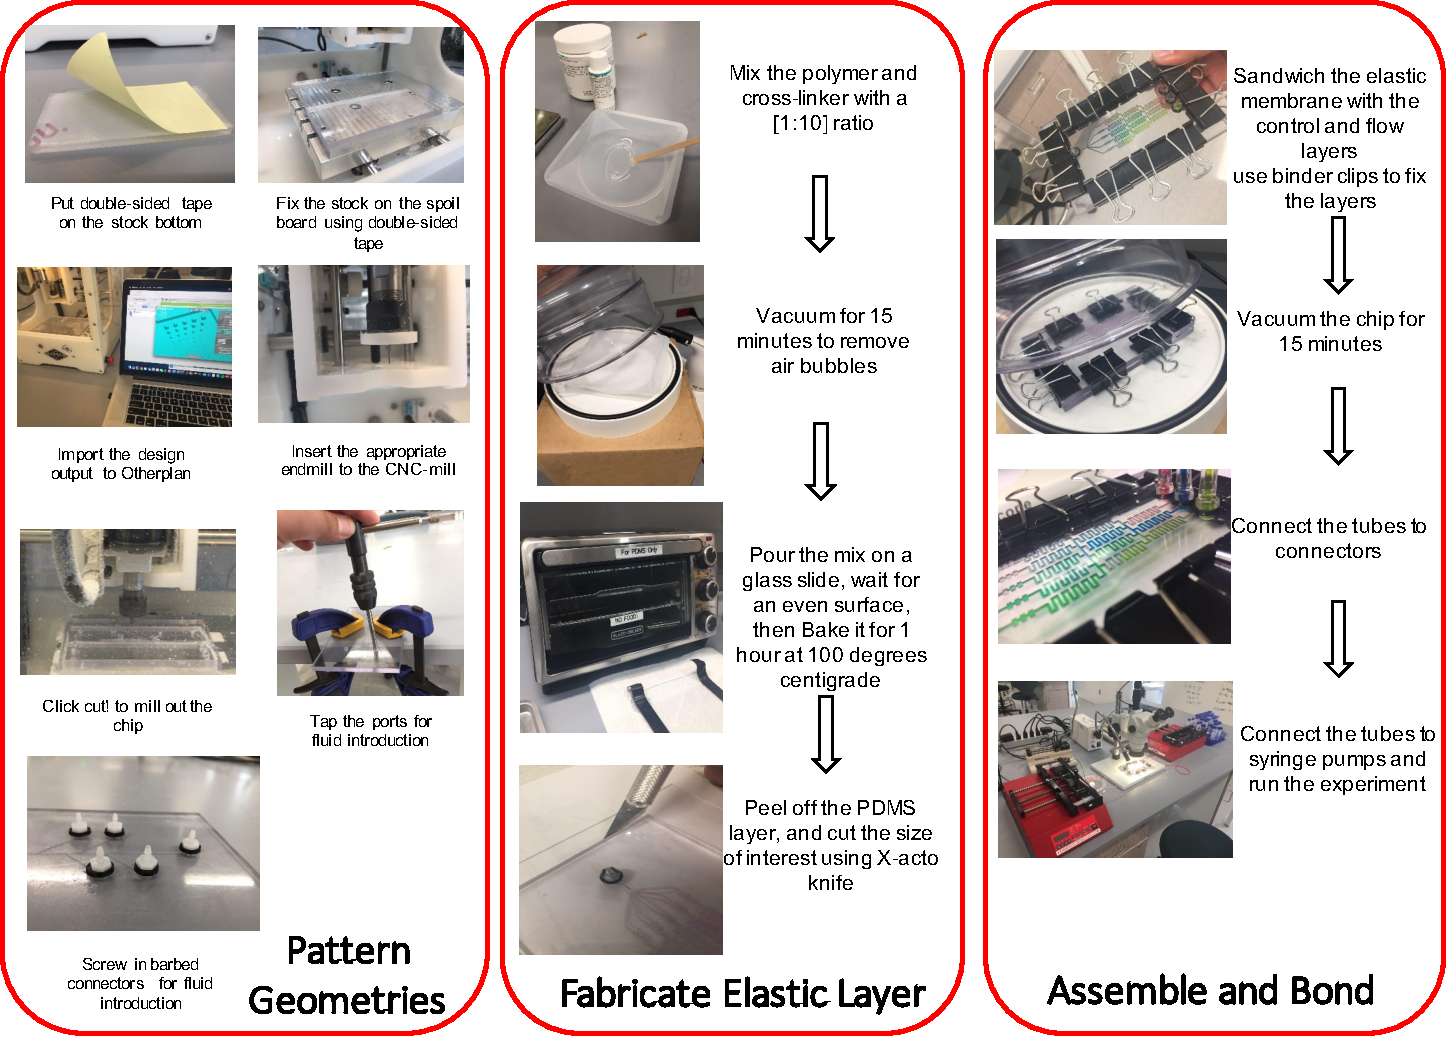
\includegraphics[width=14cm]{fabFlow.pdf}
    \medskip
  \end{minipage}\hfill
  \caption[The MakerFluidics fabrication protocol]{Workflow for fabricating microfluidics using the MakerFluidics framework.}
    \label{fig:fabFlow}
\end{figure}




\section{Experimental Control}
\label{sec:mfControl}
MakerFluidics views experimental conditions as a sequence of temporally-specified valve conditions. This necessitates a data structure consisting of an enumerated array of valve objects and a sequence of temporal specifications regarding their state. This data structure can be automatically generated by microfluidic CAD software developed in house, but it can also be created manually as a series of wait statements and valve conditions shown in Figure \ref{fig:sequence}. These valve objects are linked to the microfluidic layout provided to the fabrication software through the use of a graphical user interface (GUI).

Pneumatics are provided through an array of 3D printed syringe pumps controlled by custom firmware on an Arduino microcontroller. This microcontroller receives serial commands derived from the GUI running on a host computer. The MakerFluidics control GUI and firmware is extensible and interoperable with a conventional, solenoid-driven control infrastructure.

\begin{figure}[h]
  \begin{minipage}[t]{0.99\linewidth}\centering
    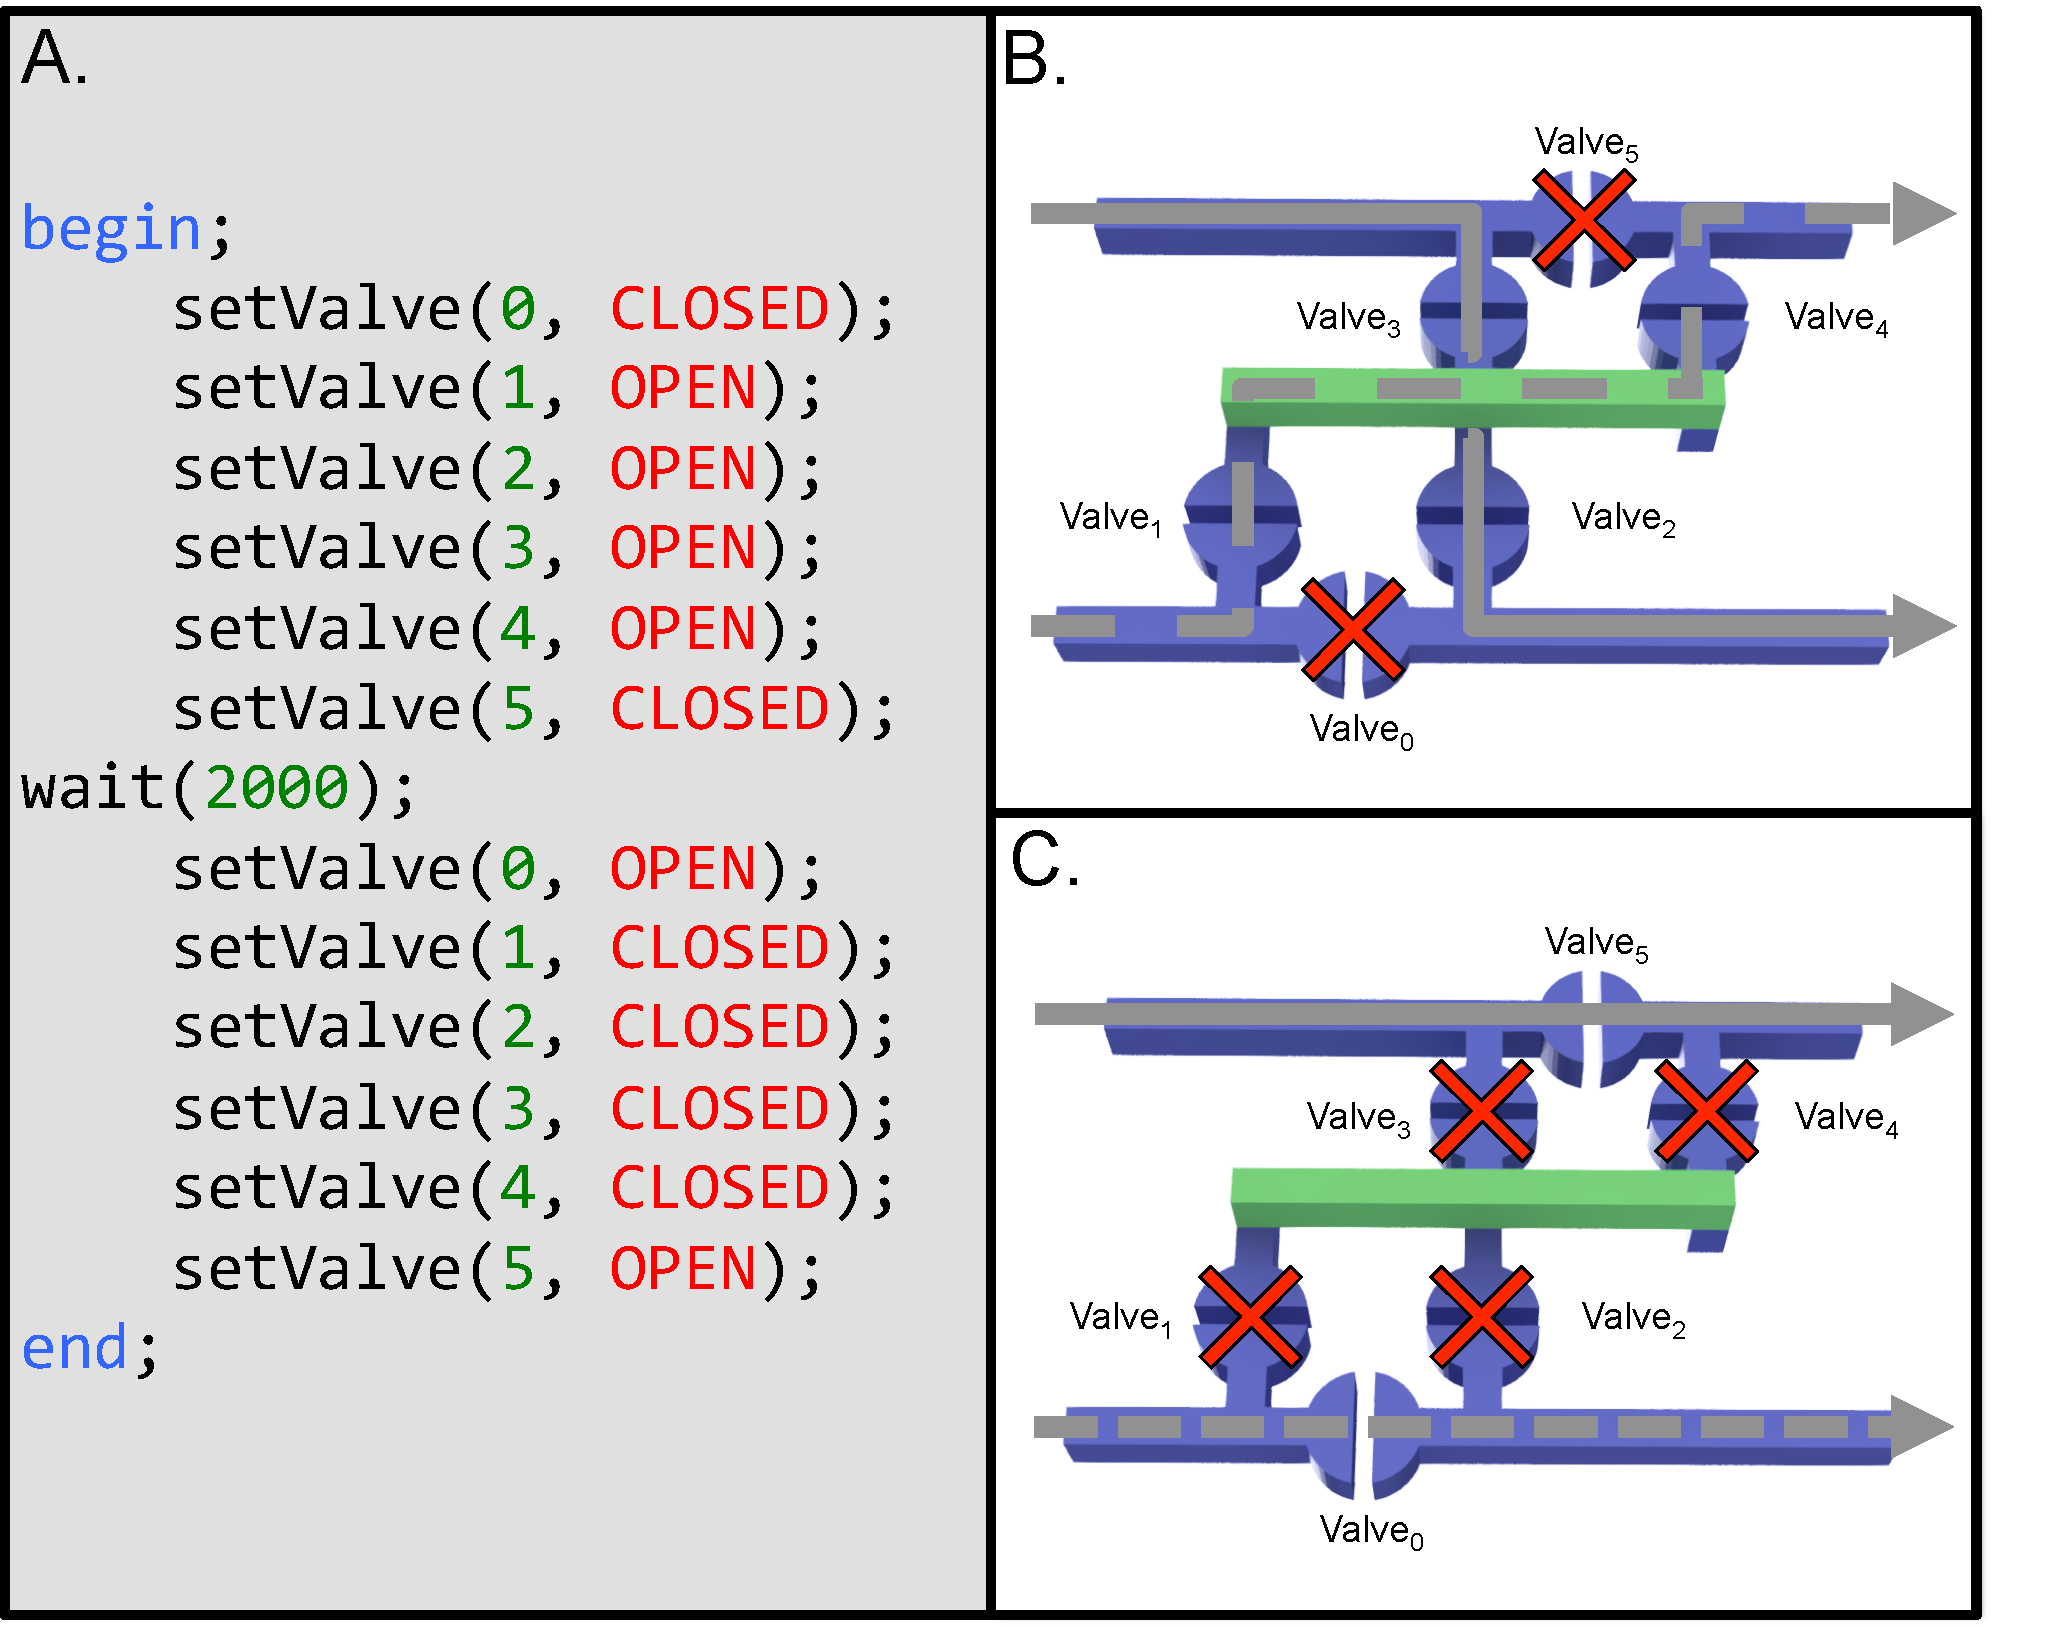
\includegraphics[width=14cm]{sequence.pdf}
    \medskip
  \end{minipage}\hfill
  \caption[Valving sequence temporal specification]{The temporal specification (A) \cite{thies2008} for a device containing six valves (B, C). The specification in (A) dictates the set of conditions in (B) to begin the assay. After 2000ms the valves change state to that shown in (C), thus affecting the movement of fluid through the device.}
    \label{fig:sequence}
\end{figure}

\section{Applicability of MakerFluidics}
\label{sec:mfApplicability}
While the collection of protocols and technologies that define MakerFluidics may seem simplistic, the relevance of the framework was demonstrated by  its ability to design, fabricate, and control a complex network of novel microfluidic primitives, as described in the subsequent chapter. Additionally the framework was used to fabricate experimentally relevant devices in industry. This work is presented in Chapter \ref{chapter:acoust}.
